\documentclass[12pt,letter]{article}\usepackage[]{graphicx}\usepackage[]{color}
%% maxwidth is the original width if it is less than linewidth
%% otherwise use linewidth (to make sure the graphics do not exceed the margin)
\makeatletter
\def\maxwidth{ %
  \ifdim\Gin@nat@width>\linewidth
    \linewidth
  \else
    \Gin@nat@width
  \fi
}
\makeatother

\definecolor{fgcolor}{rgb}{0.345, 0.345, 0.345}
\newcommand{\hlnum}[1]{\textcolor[rgb]{0.686,0.059,0.569}{#1}}%
\newcommand{\hlstr}[1]{\textcolor[rgb]{0.192,0.494,0.8}{#1}}%
\newcommand{\hlcom}[1]{\textcolor[rgb]{0.678,0.584,0.686}{\textit{#1}}}%
\newcommand{\hlopt}[1]{\textcolor[rgb]{0,0,0}{#1}}%
\newcommand{\hlstd}[1]{\textcolor[rgb]{0.345,0.345,0.345}{#1}}%
\newcommand{\hlkwa}[1]{\textcolor[rgb]{0.161,0.373,0.58}{\textbf{#1}}}%
\newcommand{\hlkwb}[1]{\textcolor[rgb]{0.69,0.353,0.396}{#1}}%
\newcommand{\hlkwc}[1]{\textcolor[rgb]{0.333,0.667,0.333}{#1}}%
\newcommand{\hlkwd}[1]{\textcolor[rgb]{0.737,0.353,0.396}{\textbf{#1}}}%

\usepackage{framed}
\makeatletter
\newenvironment{kframe}{%
 \def\at@end@of@kframe{}%
 \ifinner\ifhmode%
  \def\at@end@of@kframe{\end{minipage}}%
  \begin{minipage}{\columnwidth}%
 \fi\fi%
 \def\FrameCommand##1{\hskip\@totalleftmargin \hskip-\fboxsep
 \colorbox{shadecolor}{##1}\hskip-\fboxsep
     % There is no \\@totalrightmargin, so:
     \hskip-\linewidth \hskip-\@totalleftmargin \hskip\columnwidth}%
 \MakeFramed {\advance\hsize-\width
   \@totalleftmargin\z@ \linewidth\hsize
   \@setminipage}}%
 {\par\unskip\endMakeFramed%
 \at@end@of@kframe}
\makeatother

\definecolor{shadecolor}{rgb}{.97, .97, .97}
\definecolor{messagecolor}{rgb}{0, 0, 0}
\definecolor{warningcolor}{rgb}{1, 0, 1}
\definecolor{errorcolor}{rgb}{1, 0, 0}
\newenvironment{knitrout}{}{} % an empty environment to be redefined in TeX

\usepackage{alltt}
\usepackage{amsmath}
\usepackage{url}
\usepackage{tikz}
\usepackage{adjustbox}

\usetikzlibrary{arrows}
\usetikzlibrary{bayesnet}

\DeclareMathOperator*{\argmin}{\arg\!\min}
\DeclareMathOperator*{\argmax}{\arg\!\max}
\IfFileExists{upquote.sty}{\usepackage{upquote}}{}

\begin{document}










\section*{Introduction}
Social scientists have collected a wide and sophisticated arsenal of
ways to group similar elements of network. However, except in simplest
cases, what determines the output is the simple, iterative algorithm
of the researcher fiddling with weights until the groupings look how
she wants them to. Our methods to group similar elements depends on us
knowing what similarity means in our network. We usually don't.

When our similarity is binary, i.e. did ego nominate
alter as friend, life is easy. But, as soon as a variable has more
than two possible values then the researcher must decide how to turn
those values into similarities. Different, reasonable choices will
lead to different groupings. A careful researcher may check
her choices for robustness, but may only learn that her errors are
robust. The difficulties grow combinatorially if we decide that
a second, third, or more variable might be of some interest.

In the end, we adjust the various weights until the groupings come out
looking about right. We would have been better off just drawing what
we wanted in the first place.

We would be better off because we humans are all too good at
apprehending an assortment of things as a group than we are at
assigning importance to variables by manually assigning weights, which
we are very, very bad at.

While the interestingness of apprehended unities may vary 
unfairly between individual sociologists (not every one has Weberian gift),
we are professionally required to be interested in the way that a
collection of people groups themselves.

If we can collect information on how people group themselves, then we
can learn what counts for similarity for these people. Understanding
what similarity means for is not only scientifically interesting in
itself, it will also allow for principles prediction of how similar
collections of people will group themselves.

In this paper I discuss how to do learn about similarity using the
case of city neighborhoods. 

\subsection{Neighborhood Model Representation}
Let's imagine a very small city consisting of four blocks. We can
represent this tiny town as a network where two blocks are connected
if they face the same street. In this representation, blocks that are
kitty corner are not directly connected. We'll index the blocks as
$1$, $2$, $3$, and $4$.

\begin{figure}[h]
\centering
\tikz{
\draw[help lines] (0,0) grid (2,2);
\node at (0.5, 0.5) {3} ;
\node at (1.5, 1.5) {2} ;
\node at (0.5, 1.5) {1} ;
\node at (1.5, 0.5) {4} ;
}
\end{figure}

\begin{figure}[h]
\centering

\tikz{ %
  \node[latent] (1) {$1$} ; %
  \node[latent, below left=of 1] (2) {$2$} ; %
  \node[latent, below right=of 1] (3) {$3$} ; %
  \node[latent, below left=of 3] (4) {$4$} ; %
  \edge[-] {2,3} {1} ; %
  \edge[-] {2,3} {4} ; %
}

\end{figure}

Suppose that, in our city, there are two neighborhoods. Each block
belongs to either one or the other of these neighborhoods. Neighboring
blocks that are similar are more apt to belong to the same
neighborhood and neighboring blocks that are different are more apt to
belong to different neighborhoods.

We want similar blocks to belong to the same
neighborhood. One way to formalize this desire is to score every
possible pattern of neighborhood labels in such a way that our
preferred patterns have the best score.

First, we need some more precise terms. Let the two neighborhoods be
called $0$ and $1$. A block belongs to either neighborhood $0$ or
$1$, and we will denote this membership as $y_i$, so that $y_1=0$ is
equivalent to saying that block $1$ belongs to the $0$
neighborhood. Let the similarity between blocks $i$ and $j$ be called
$\phi_{i,j}$.

\begin{figure}[!h]
\centering

\tikz{ %
  \node[latent] (1) {$y_1$} ; %
  \node[latent, below left=of 1] (2) {$y_2$} ; %
  \node[latent, below right=of 1] (3) {$y_3$} ; %
  \node[latent, below left=of 3] (4) {$y_4$} ; %
  \factor[below left=of 1] {1-2} {$\phi_{1,2}$} {} {} ;
  \factor[below right=of 1] {1-3} {$\phi_{1,3}$} {} {} ;
  \factor[below right=of 2] {2-4} {$\phi_{2,4}$} {} {} ;
  \factor[below left=of 3] {3-4} {$\phi_{3,4}$} {} {} ;
  \factoredge[-] {1} {1-2} {2} ; %
  \factoredge[-] {1} {1-3} {3} ; %
  \factoredge[-] {2} {2-4} {4} ; %
  \factoredge[-] {3} {3-4} {4} ; %
  %\edge[-] {2,3} {4} ; %
}

\end{figure}


Let a particular pattern of assignment of blocks to neighborhoods
be called $\mathbf{y}$.  The score of $\mathbf{y}$ will be
$\operatorname{E}(\mathbf{y})$\footnote{$\operatorname{E}$ as in
  energy not expectation} which will take the following form:

\begin{align}
\operatorname{E}(\mathbf{y}) = \sum_{<i,j>}^{\mathcal{N}}\epsilon_{i,j}(y_i,y_j,\phi_{i,j})
\end{align}

Where $<i,j>$ indexes a pair of neighboring blocks, and where $i < j$.
$\mathcal{N}$ are all these indices of neighboring blocks. The
$\epsilon_{i,j}$ function is 

\begin{equation}
\epsilon_{i,j}(y_i,y_j,\phi_{i,j}) = \begin{cases}
  0 &y_i = y_j \\
  \phi_{i,j} &y_i \neq y_j
\end{cases}
\end{equation}

Suppose that we want our preferred neighborhood assignment to have the
lowest score. If our similarity measures $\phi_{i,j}$ are positive
when blocks are similar and negative when blocks are different, then
we will encourage similar, neighboring blocks to belong to the same
neighborhood. 

Let our city have the following $\phi$'s.

\begin{align*}
&\phi_{1,2} = 1 \\
&\phi_{1,3} = -1 \\
&\phi_{2,4} = -1 \\
&\phi_{3,4} = 1
\end{align*} 

\noindent
If we now score every possible pattern of neighborhood labels, we will
find that the lowest scoring assignments are ones that put blocks $1$
and $2$ in one neighborhood and $3$ and $4$ in the other (Table
\ref{table:lowest}, Table \ref{table:energy}). By choosing the right
$\phi$'s we can have made our preferred pattern have the lowest scores.

\begin{table}
\centering
  \begin{tabular}{cc}
      \tikz{ %
        \node[latent] (1) {$y_1$} ; %
        \node[latent, below left=of 1] (2) {$y_2$} ; %
        \node[latent, fill=black, below right=of 1] (3) {\textcolor{white}{$y_3$}} ; %
        \node[latent, fill=black, below left=of 3] (4) {\textcolor{white}{$y_4$}} ; %
        \factor[below left=of 1] {1-2} {$1$} {} {} ;
        \factor[below right=of 1] {1-3} {$-1$} {} {} ;
        \factor[below right=of 2] {2-4} {$-1$} {} {} ;
        \factor[below left=of 3] {3-4} {$1$} {} {} ;
        \factoredge[-] {1} {1-2} {2} ; %
        \factoredge[-] {1} {1-3} {3} ; %
        \factoredge[-] {2} {2-4} {4} ; %
        \factoredge[-] {3} {3-4} {4} ; %
      } 
    &
      \tikz{ %
        \node[latent, fill=black] (1) {\textcolor{white}{$y_1$}} ; %
        \node[latent, fill=black, below left=of 1] (2) {\textcolor{white}{$y_2$}} ; %
        \node[latent, below right=of 1] (3) {$y_3$} ; %
        \node[latent, below left=of 3] (4) {$y_4$} ; %
        \factor[below left=of 1] {1-2} {$1$} {} {} ;
        \factor[below right=of 1] {1-3} {$-1$} {} {} ;
        \factor[below right=of 2] {2-4} {$-1$} {} {} ;
        \factor[below left=of 3] {3-4} {$1$} {} {} ;
        \factoredge[-] {1} {1-2} {2} ; %
        \factoredge[-] {1} {1-3} {3} ; %
        \factoredge[-] {2} {2-4} {4} ; %
        \factoredge[-] {3} {3-4} {4} ; %
      } 
    \\
  \end{tabular}
  \caption{Preferred Assignment: If $y_i = 0$, the block is colored
    white. If $y_i = 1$, the block is black.}
  \label{table:lowest}
\end{table}

\begin{table}[h]
\begin{tabular}{cl}
  \\
  $\operatorname{E}(\mathbf{y}) = -2$
  & 
  \begin{tabular}{cccc}
    \scalebox{0.5}{
      \tikz{ %
        \node[latent] (1) {$0$} ; %
        \node[latent, below left=of 1] (2) {$0$} ; %
        \node[latent, fill=black, below right=of 1] (3) {\textcolor{white}{$1$}} ; %
        \node[latent, fill=black, below left=of 3] (4) {\textcolor{white}{$1$}} ; %
        \factor[below left=of 1] {1-2} {} {} {} ;
        \factor[below right=of 1] {1-3} {} {} {} ;
        \factor[below right=of 2] {2-4} {} {} {} ;
        \factor[below left=of 3] {3-4} {} {} {} ;
        \factoredge[-] {1} {1-2} {2} ; %
        \factoredge[-] {1} {1-3} {3} ; %
        \factoredge[-] {2} {2-4} {4} ; %
        \factoredge[-] {3} {3-4} {4} ; %
        %\edge[-] {2,3} {4} ; %
      } 
    }
    &
    \scalebox{0.5}{
      \tikz{ %
        \node[latent, fill=black] (1) {\textcolor{white}{$8$}} ; %
        \node[latent, fill=black, below left=of 1] (2) {\textcolor{white}{$1$}} ; %
        \node[latent, below right=of 1] (3) {$0$} ; %
        \node[latent, below left=of 3] (4) {$0$} ; %
        \factor[below left=of 1] {1-2} {} {} {} ;
        \factor[below right=of 1] {1-3} {} {} {} ;
        \factor[below right=of 2] {2-4} {} {} {} ;
        \factor[below left=of 3] {3-4} {} {} {} ;
        \factoredge[-] {1} {1-2} {2} ; %
        \factoredge[-] {1} {1-3} {3} ; %
        \factoredge[-] {2} {2-4} {4} ; %
        \factoredge[-] {3} {3-4} {4} ; %
        %\edge[-] {2,3} {4} ; %
      } 
    }
    \\
  \end{tabular}
  \\ \hline

  $\operatorname{E}(\mathbf{y}) = 0$
  &
  \begin{tabular}{cccc}
    \scalebox{0.5}{
      \tikz{ %
        \node[latent, fill=black] (1) {\textcolor{white}{$1$}} ; %
        \node[latent, fill=black, below left=of 1] (2) {\textcolor{white}{$1$}} ; %
        \node[latent, fill=black, below right=of 1] (3) {\textcolor{white}{$1$}} ; %
        \node[latent, fill=black, below left=of 3] (4) {\textcolor{white}{$1$}} ; %
        \factor[below left=of 1] {1-2} {} {} {} ;
        \factor[below right=of 1] {1-3} {} {} {} ;
        \factor[below right=of 2] {2-4} {} {} {} ;
        \factor[below left=of 3] {3-4} {} {} {} ;
        \factoredge[-] {1} {1-2} {2} ; %
        \factoredge[-] {1} {1-3} {3} ; %
        \factoredge[-] {2} {2-4} {4} ; %
        \factoredge[-] {3} {3-4} {4} ; %
        %\edge[-] {2,3} {4} ; %
      } 
    }
    \\
    \scalebox{0.5}{
      \tikz{ %
        \node[latent] (1) {$6$} ; %
        \node[latent, fill=black, below left=of 1] (2) {\textcolor{white}{$1$}} ; %
        \node[latent, fill=black, below right=of 1] (3) {\textcolor{white}{$1$}} ; %
        \node[latent, fill=black, below left=of 3] (4) {\textcolor{white}{$1$}} ; %
        \factor[below left=of 1] {1-2} {} {} {} ;
        \factor[below right=of 1] {1-3} {} {} {} ;
        \factor[below right=of 2] {2-4} {} {} {} ;
        \factor[below left=of 3] {3-4} {} {} {} ;
        \factoredge[-] {1} {1-2} {2} ; %
        \factoredge[-] {1} {1-3} {3} ; %
        \factoredge[-] {2} {2-4} {4} ; %
        \factoredge[-] {3} {3-4} {4} ; %
        %\edge[-] {2,3} {4} ; %
      } 
    }
    &
    \scalebox{0.5}{
      \tikz{ %
        \node[latent, fill=black] (1) {\textcolor{white}{$1$}} ; %
        \node[latent, below left=of 1] (2) {$0$} ; %
        \node[latent, fill=black, below right=of 1] (3) {\textcolor{white}{$1$}} ; %
        \node[latent, fill=black, below left=of 3] (4) {\textcolor{white}{$1$}} ; %
        \factor[below left=of 1] {1-2} {} {} {} ;
        \factor[below right=of 1] {1-3} {} {} {} ;
        \factor[below right=of 2] {2-4} {} {} {} ;
        \factor[below left=of 3] {3-4} {} {} {} ;
        \factoredge[-] {1} {1-2} {2} ; %
        \factoredge[-] {1} {1-3} {3} ; %
        \factoredge[-] {2} {2-4} {4} ; %
        \factoredge[-] {3} {3-4} {4} ; %
        %\edge[-] {2,3} {4} ; %
      } 
    }
    &
    \scalebox{0.5}{
      \tikz{ %
        \node[latent, fill=black] (1) {\textcolor{white}{$1$}} ; %
        \node[latent, fill=black, below left=of 1] (2) {\textcolor{white}{$1$}} ; %
        \node[latent, fill=black, below right=of 1] (3) {\textcolor{white}{$1$}} ; %
        \node[latent, below left=of 3] (4) {$0$} ; %
        \factor[below left=of 1] {1-2} {} {} {} ;
        \factor[below right=of 1] {1-3} {} {} {} ;
        \factor[below right=of 2] {2-4} {} {} {} ;
        \factor[below left=of 3] {3-4} {} {} {} ;
        \factoredge[-] {1} {1-2} {2} ; %
        \factoredge[-] {1} {1-3} {3} ; %
        \factoredge[-] {2} {2-4} {4} ; %
        \factoredge[-] {3} {3-4} {4} ; %
        %\edge[-] {2,3} {4} ; %
      }
    }
    &
    \scalebox{0.5}{
      \tikz{ %
        \node[latent, fill=black] (1) {\textcolor{white}{$1$}} ; %
        \node[latent, fill=black, below left=of 1] (2) {\textcolor{white}{$1$}} ; %
        \node[latent, below right=of 1] (3) {$0$} ; %
        \node[latent, fill=black, below left=of 3] (4) {\textcolor{white}{$1$}} ; %
        \factor[below left=of 1] {1-2} {} {} {} ;
        \factor[below right=of 1] {1-3} {} {} {} ;
        \factor[below right=of 2] {2-4} {} {} {} ;
        \factor[below left=of 3] {3-4} {} {} {} ;
        \factoredge[-] {1} {1-2} {2} ; %
        \factoredge[-] {1} {1-3} {3} ; %
        \factoredge[-] {2} {2-4} {4} ; %
        \factoredge[-] {3} {3-4} {4} ; %
        %\edge[-] {2,3} {4} ; %
      } 
    }
    \\
    \scalebox{0.5}{
      \tikz{ %
        \node[latent] (1) {$0$} ; %
        \node[latent, fill=black, below left=of 1] (2) {\textcolor{white}{$1$}} ; %
        \node[latent, fill=black, below right=of 1] (3) {\textcolor{white}{$1$}} ; %
        \node[latent, below left=of 3] (4) {$0$} ; %
        \factor[below left=of 1] {1-2} {} {} {} ;
        \factor[below right=of 1] {1-3} {} {} {} ;
        \factor[below right=of 2] {2-4} {} {} {} ;
        \factor[below left=of 3] {3-4} {} {} {} ;
        \factoredge[-] {1} {1-2} {2} ; %
        \factoredge[-] {1} {1-3} {3} ; %
        \factoredge[-] {2} {2-4} {4} ; %
        \factoredge[-] {3} {3-4} {4} ; %
        %\edge[-] {2,3} {4} ; %
      }
    }
    &
    \scalebox{0.5}{
      \tikz{ %
        \node[latent, fill=black] (1) {\textcolor{white}{$1$}} ; %
        \node[latent, below left=of 1] (2) {$0$} ; %
        \node[latent, below right=of 1] (3) {$0$} ; %
        \node[latent, fill=black, below left=of 3] (4) {\textcolor{white}{$1$}} ; %
        \factor[below left=of 1] {1-2} {} {} {} ;
        \factor[below right=of 1] {1-3} {} {} {} ;
        \factor[below right=of 2] {2-4} {} {} {} ;
        \factor[below left=of 3] {3-4} {} {} {} ;
        \factoredge[-] {1} {1-2} {2} ; %
        \factoredge[-] {1} {1-3} {3} ; %
        \factoredge[-] {2} {2-4} {4} ; %
        \factoredge[-] {3} {3-4} {4} ; %
        %\edge[-] {2,3} {4} ; %
      } 
    }
    \\
    \scalebox{0.5}{
      \tikz{ %
        \node[latent, fill=black] (1) {\textcolor{white}{$1$}} ; %
        \node[latent, below left=of 1] (2) {$0$} ; %
        \node[latent, below right=of 1] (3) {$0$} ; %
        \node[latent, below left=of 3] (4) {$0$} ; %
        \factor[below left=of 1] {1-2} {} {} {} ;
        \factor[below right=of 1] {1-3} {} {} {} ;
        \factor[below right=of 2] {2-4} {} {} {} ;
        \factor[below left=of 3] {3-4} {} {} {} ;
        \factoredge[-] {1} {1-2} {2} ; %
        \factoredge[-] {1} {1-3} {3} ; %
        \factoredge[-] {2} {2-4} {4} ; %
        \factoredge[-] {3} {3-4} {4} ; %
        %\edge[-] {2,3} {4} ; %
      }
    }
    &
    \scalebox{0.5}{
      \tikz{ %
        \node[latent] (1) {$0$} ; %
        \node[latent, fill=black, below left=of 1] (2) {\textcolor{white}{$1$}} ; %
        \node[latent, below right=of 1] (3) {$0$} ; %
        \node[latent, below left=of 3] (4) {$0$} ; %
        \factor[below left=of 1] {1-2} {} {} {} ;
        \factor[below right=of 1] {1-3} {} {} {} ;
        \factor[below right=of 2] {2-4} {} {} {} ;
        \factor[below left=of 3] {3-4} {} {} {} ;
        \factoredge[-] {1} {1-2} {2} ; %
        \factoredge[-] {1} {1-3} {3} ; %
        \factoredge[-] {2} {2-4} {4} ; %
        \factoredge[-] {3} {3-4} {4} ; %
        %\edge[-] {2,3} {4} ; %
      } 
    }
    &
    \scalebox{0.5}{
      \tikz{ %
        \node[latent] (1) {$0$} ; %
        \node[latent, below left=of 1] (2) {$0$} ; %
        \node[latent, below right=of 1] (3) {$0$} ; %
        \node[latent, fill=black, below left=of 3] (4) {\textcolor{white}{$1$}} ; %
        \factor[below left=of 1] {1-2} {} {} {} ;
        \factor[below right=of 1] {1-3} {} {} {} ;
        \factor[below right=of 2] {2-4} {} {} {} ;
        \factor[below left=of 3] {3-4} {} {} {} ;
        \factoredge[-] {1} {1-2} {2} ; %
        \factoredge[-] {1} {1-3} {3} ; %
        \factoredge[-] {2} {2-4} {4} ; %
        \factoredge[-] {3} {3-4} {4} ; %
        %\edge[-] {2,3} {4} ; %
      } 
    }
    &
    \scalebox{0.5}{
      \tikz{ %
        \node[latent] (1) {$0$} ; %
        \node[latent, below left=of 1] (2) {$0$} ; %
        \node[latent, fill=black, below right=of 1] (3) {\textcolor{white}{$1$}} ; %
        \node[latent, below left=of 3] (4) {$0$} ; %
        \factor[below left=of 1] {1-2} {} {} {} ;
        \factor[below right=of 1] {1-3} {} {} {} ;
        \factor[below right=of 2] {2-4} {} {} {} ;
        \factor[below left=of 3] {3-4} {} {} {} ;
        \factoredge[-] {1} {1-2} {2} ; %
        \factoredge[-] {1} {1-3} {3} ; %
        \factoredge[-] {2} {2-4} {4} ; %
        \factoredge[-] {3} {3-4} {4} ; %
        %\edge[-] {2,3} {4} ; %
      } 
    }
    \\
    % All Zeros %
    \scalebox{0.5}{
      \tikz{ %
        \node[latent] (1) {$0$} ; %
        \node[latent, below left=of 1] (2) {$0$} ; %
        \node[latent, below right=of 1] (3) {$0$} ; %
        \node[latent, below left=of 3] (4) {$0$} ; %
        \factor[below left=of 1] {1-2} {} {} {} ;
        \factor[below right=of 1] {1-3} {} {} {} ;
        \factor[below right=of 2] {2-4} {} {} {} ;
        \factor[below left=of 3] {3-4} {} {} {} ;
        \factoredge[-] {1} {1-2} {2} ; %
        \factoredge[-] {1} {1-3} {3} ; %
        \factoredge[-] {2} {2-4} {4} ; %
        \factoredge[-] {3} {3-4} {4} ; %
        %\edge[-] {2,3} {4} ; %
      } 
    }
    \\
    \end{tabular}
  \\ \hline
  % Mismatched %
  $\operatorname{E}(\mathbf{y}) = 2$
  &
  \begin{tabular}{cccc}
    \scalebox{0.5}{
      \tikz{ %
        \node[latent] (1) {$0$} ; %
        \node[latent, fill=black, below left=of 1] (2) {\textcolor{white}{$1$}} ; %
        \node[latent, below right=of 1] (3) {$0$} ; %
        \node[latent, fill=black, below left=of 3] (4) {\textcolor{white}{$1$}} ; %
        \factor[below left=of 1] {1-2} {} {} {} ;
        \factor[below right=of 1] {1-3} {} {} {} ;
        \factor[below right=of 2] {2-4} {} {} {} ;
        \factor[below left=of 3] {3-4} {} {} {} ;
        \factoredge[-] {1} {1-2} {2} ; %
        \factoredge[-] {1} {1-3} {3} ; %
        \factoredge[-] {2} {2-4} {4} ; %
        \factoredge[-] {3} {3-4} {4} ; %
        %\edge[-] {2,3} {4} ; %
      }
    }
    &
    \scalebox{0.5}{
      \tikz{ %
        \node[latent, fill=black] (1) {\textcolor{white}{$1$}} ; %
        \node[latent, below left=of 1] (2) {$0$} ; %
        \node[latent, fill=black, below right=of 1] (3) {\textcolor{white}{$1$}} ; %
        \node[latent, below left=of 3] (4) {$0$} ; %
        \factor[below left=of 1] {1-2} {} {} {} ;
        \factor[below right=of 1] {1-3} {} {} {} ;
        \factor[below right=of 2] {2-4} {} {} {} ;
        \factor[below left=of 3] {3-4} {} {} {} ;
        \factoredge[-] {1} {1-2} {2} ; %
        \factoredge[-] {1} {1-3} {3} ; %
        \factoredge[-] {2} {2-4} {4} ; %
        \factoredge[-] {3} {3-4} {4} ; %
        %\edge[-] {2,3} {4} ; %
      }
    }
    \\
  \end{tabular}
\end{tabular}

\caption{Scores of Neighborhood Assignments}
\label{table:energy}
\end{table}

\subsection{Learning similarities}
Suppose we knew that we wanted some particular pattern of
neighborhoods, but we didn't what similarity scores, $\phi$'s would
give that pattern the lowest score. In order to find the $phi$'s we
might start with a likely looking set of $\phi$'s, and check that
these similarities gave the preferred pattern the best score.

For small networks, we could check the scores for each individual
pattern, but this exhaustive strategy becomes quickly impractical
for larger cities. With two possible neighborhoods, the number of
possible assignments is $2^N$ where N is the number of blocks. This
permutational explosion means that for even small cities, we cannot
possibly check every possible neighborhood assignment in human-scale
time.

\subsubsection{Network Methods}
Fortunately, researchers, largely in the field of computer vision,
have developed methods to quickly find the lowest scoring assignment
for problems like ours. This work traces back to a 1986 paper by
Greig, Porteous, and Sehult, where they demonstrated that finding
lowest scoring assignment for a two neighborhood case was equivalent
to solving the problem of finding the minimum cut of a
network.\cite{greig_exact_1989}

In that paper, the authors set up an scoring problem that is slightly
different than ours. In addition to terms that depended upon pairs of
neighbors, their score also included terms for individual nodes.

\begin{align}
\operatorname{E}(\mathbf{y}) = \sum_i\epsilon_i(y_i) + \sum_{<i
  j>}^{\mathcal{N}}\epsilon_{i,j}(y_i,y_j,\phi_{i,j})
\end{align}

\noindent
The node terms were of one of two forms, either

\begin{equation}
\epsilon_{i}(y_i) = \begin{cases}
  0 &y_i = 0 \\
  \phi_{i} \geq 0 &y_i = 1
\end{cases}
\end{equation}

\noindent
or 

\begin{equation}
\epsilon_{i}(y_i) = \begin{cases}
  \phi_{i} \geq 0 &y_i = 0 \\
  0 &y_i = 1
\end{cases}
\end{equation}

\noindent
They had the same form of $\epsilon_{i,j}$ as we do

\begin{equation}
\epsilon_{i,j}(y_i,y_j,\phi_{i,j}) = \begin{cases}
  0 &y_i = y_j \\
  \phi_{i,j} &y_i \neq y_j
\end{cases}
\end{equation}

\noindent
but unlike us, $\phi_{i,j} \geq 0$ for all $<i, j>$ in $\mathcal{N}$. 

One of their networks could look like this

\begin{figure}[!h]
\centering

\tikz{ %
  \node[latent] (1) {$y_1$} ; %
  \node[latent, below left=of 1] (2) {$y_2$} ; %
  \node[latent, below right=of 1] (3) {$y_3$} ; %
  \node[latent, below left=of 3] (4) {$y_4$} ; %
  \factor[below left=of 1] {1-2} {$1$} {} {} ;
  \factor[below right=of 1] {1-3} {$1$} {} {} ;
  \factor[below right=of 2] {2-4} {$1$} {} {} ;
  \factor[below left=of 3] {3-4} {$1$} {} {} ;
  \factoredge[-] {1} {1-2} {2} ; %
  \factoredge[-] {1} {1-3} {3} ; %
  \factoredge[-] {2} {2-4} {4} ; %
  \factoredge[-] {3} {3-4} {4} ; %
  %\edge[-] {2,3} {4} ; %
}

\end{figure}

Based on this undirected network, Greig and his co-authors constructed
a special, directed network where every edge has a cost associated
with it. For every variable $y_i$ in the undirected network, the
directed network contains a node $z_i$.  For every edge $(y_i, y_j)$ in the
undirected network, they introduced a directed edge from $z_i$ to $z_j$ and
another from $z_j$ to $z_i$ with associated costs of $\phi_{i,j}$.

In addition to the original nodes, they also introduced two special
nodes: a source node called $s$ and a target, or sink, node called
$t$. If $\epsilon_i(0) = 0$ then there would be a directed edge from
$s$ to the $i$th node. If $\epsilon_i(1) = 0$ then there would be
directed edge from the $i$th node to $t$. Networks like this are
called s-t networks.

Suppose that $\epsilon_1(1)=2$, $\epsilon_2(0)=1$, $\epsilon_3(1)=3$,
and $\epsilon_4(0)=3$. The corresponding directed network is shown in
Figure \ref{fig:directed}. 

\begin{figure}[!h]
\centering

\begin{tikzpicture}[auto, >= stealth', shorten >= 1pt, node
    distance=2cm, thick]
\tikzset{vertex/.style = {shape=circle, draw, minimum size = 1.5em}}
\tikzset{Dedge/.style = {->}}
\tikzset{Uedge/.style = {<->}}

\node[vertex, above=of 1] (0) {$s$} ; %
\node[vertex] (1) {$y_1$} ; %
\node[vertex, below left=of 1] (2) {$y_2$} ; %
\node[vertex, below right=of 1] (3) {$y_3$} ; %
\node[vertex, below left=of 3] (4) {$y_4$} ; %
\node[vertex, below=of 4] (5) {$t$} ; %
\path
  (0) edge [Dedge] node {2} (1)
  (0) edge [Dedge, bend left] node[right] {3} (3)
  (1) edge [Uedge] node {1} (2) 
  (1) edge [Uedge] node {1} (3) 
  (2) edge [Uedge] node {1} (4) 
  (3) edge [Uedge] node {1} (4) 
  (2) edge [Dedge, bend right] node[left] {1} (5)
  (4) edge [Dedge] node {3} (5)  ;

\end{tikzpicture}
\caption{S-T Network}
\label{fig:directed}
\end{figure}

We must now introduce some terms. First, to `cut' a network is to
remove edges from the network so that the network is split into two
unconnected, smaller networks. Second, an `s-t cut' is a cut on a s-t
network that causes the source node and target node to end up in
separate, unconnected networks. Finally, a `minimum cut' is an s-t cut
where the sum of cost associated with the removed edges is as small as
any other possible s-t cut. 

In our example, removing the edges $(z_2, t)$ and $(z_4, t)$ is an s-t
cut, but not the minimum cut. The minimum cut would be removing edges
$(z_1, z_2)$ and $(z_3, z_4)$ (Figure \ref{fig:mincut}).

\begin{figure}[!h]
\centering

\begin{tikzpicture}[auto, >= stealth', shorten >= 1pt, node
    distance=2cm, thick]
\tikzset{vertex/.style = {shape=circle, draw, minimum size = 1.5em}}
\tikzset{Dedge/.style = {->}}
\tikzset{Uedge/.style = {<->}}

\node[vertex, above=of 1] (0) {$s$} ; %
\node[vertex] (1) {$y_1$} ; %
\node[vertex, below left=of 1] (2) {$y_2$} ; %
\node[vertex, below right=of 1] (3) {$y_3$} ; %
\node[vertex, below left=of 3] (4) {$y_4$} ; %
\node[vertex, below=of 4] (5) {$t$} ; %
\path
  (0) edge [Dedge] node {2} (1)
  (0) edge [Dedge, bend left] node[right] {3} (3)
  (1) edge [Uedge] node {1} (3) 
  (2) edge [Uedge] node {1} (4) 
  (2) edge [Dedge, bend right] node[left] {1} (5)
  (4) edge [Dedge] node {3} (5)  ;

\end{tikzpicture}
\caption{Minimum Cut}
\label{fig:mincut}
\end{figure}

Every s-t cut can be mapped onto a pattern of neighborhood block
labels by letting $y_i = 1$ if node $z_i$ ends up in the $t$
subnetwork and $y_i = 0$ otherwise. Greig and his coauthors
demonstrated that the minimum cut of their constructed s-t network
always corresponded to the minimum scoring pattern of block
assignment.

Because computer scientists have known how to solve the minimum cut
problem swiftly since the 1950s, this meant that a large class of
network configurations problems were now tractable. Instead of
checking every possible pattern out of exponentially possibilities, we
can now find the best scoring pattern directly and
quickly.\cite{ford_maximal_1956}

In particular, if we want to see if a certain set of similarities,
$\phi's$ gives a preferred pattern of neighborhood labels a lower
score than any other pattern, we can apply Greig's approach. If the
minimum cut of the associated s-t network corresponds to our preferred
pattern, then we know that a set of similarities gives us our
preferred pattern the lowest score. If the minimum cut corresponds to
some other pattern, then we know that these $\phi$'s do not give our
preferred pattern the lowest score.

\paragraph{Submodularity}
Greig and his coauthors' original result only applied to scoring functions 
where blocks could belong to only one of two classes and where the
scoring function had an important property called submodularity.  A
submodular scoring function would be one where $\epsilon_{i,j}(0,0) +
\epsilon_{i,j}(1,1) \leq \epsilon_{i,j}(0,1) + \epsilon_{i,j}(1,0)$
for all $i,j$ in $\mathcal{N}$. Our scoring function is decisively not
submodular because we want it to cost more to put together very
dissimilar neighboring blocks than to assign them to them to different
neighborhoods. That is, for very dissimilar blocks we want it to hold
that $\epsilon_{i,j}(0,0) + \epsilon_{i,j}(1,1) \boldsymbol{>}
\epsilon_{i,j}(0,1) + \epsilon_{i,j}(1,0)$.

Since we don't have a submodular scoring functions and often will have
more than two neighborhood names, we can't use the minimum cuts
algorithm directly to find the lowest scoring neighborhood
pattern. However, since the 1980s computers scientists have developed
other graph cutting methods that allow us to find approximate
solutions to multi-label non-submodular scoring problems like ours
\cite{something}.

\subsection{Learning similarities}
These network methods mean that we can quickly check if a
particular set of inter-block similarities gives a preferred
neighborhood pattern the best score. We will now describe how to use
this to efficiently inter-block similarities that will give a
preferred pattern the lowest score.

We will make our lives easier by only considering simple, linear
similarity terms. As before, the scoring function will be

\begin{align}
\operatorname{E}(\mathbf{y}) = \sum_{<i,j>}^{\mathcal{N}}\epsilon_{i,j}(y_i,y_j,\phi_{i,j})
\end{align}

\noindent
and

\begin{equation}
\epsilon_{i,j}(y_i,y_j,\phi_{i,j}) = \begin{cases}
  0 &y_i = y_j \\
  \phi_{i,j} &y_i \neq y_j
\end{cases}
\end{equation}

\noindent
but now, let the similarity term $\phi_{i,j}$ be the weighted sum of
observed similarities between block $i$ and $j$. 

\begin{align}
\phi_{i,j} = w_0 + w_1s_{1,i,j} + w_2s_{2,i,j} + ... + w_ns_{n,i,j}
\end{align} 

\noindent
An observed inter-block similarity could be absolute difference in
population, or dummy variable indicating whether the blocks are
separated by a railroad, or similar.

\noindent

With this form, learning a scoring function means finding weights
that give a better score to our preferred pattern of neighborhood
assignments than any other pattern. In other words, we want to find
some weights, $\mathbf{w}$, that solves this system of linear
equations:

\begin{align*}
\operatorname{E}(\mathbf{y}_1, \mathbf{s}, \mathbf{w})
&\geq \operatorname{E}(\mathbf{y}^*, \mathbf{s}, \mathbf{w}) \\
\operatorname{E}(\mathbf{y}_2, \mathbf{s}, \mathbf{w})
&\geq \operatorname{E}(\mathbf{y}^*, \mathbf{s}, \mathbf{w}) \\
&\ldots \\
\operatorname{E}(\mathbf{y}_{M-1}, \mathbf{s}, \mathbf{w})
&\geq \operatorname{E}(\mathbf{y}^*, \mathbf{s}, \mathbf{w}) \\
\operatorname{E}(\mathbf{y}_{M}, \mathbf{s}, \mathbf{w})
&\geq \operatorname{E}(\mathbf{y}^*, \mathbf{s}, \mathbf{w})
\end{align*}

Where $\mathbf{y}^*$ is our preferred pattern, M is the number of
possible neighborhood patterns, and $\mathbf{s}$ are the similarities
between blocks.

\subsubsection{Specifying a unique solution}
In order to use some convenient machinery, we will modify the learning
problem somewhat. These modifications will only act to specify a
particular solution to the system of inequalities. Any solution to the
modified problems is also a solution to the system of inequalities and
if there is solution to the system of inequalities there will be a
solution to the modified problems.

First, observe that if a set of weights gives the preferred assignment
a lower score than any other assignment, there is some difference
between the score of the preferred assignment and the score of the
next best scoring assignment. Call this difference the `margin.' Our
first modification to the learning problem is that we now seek the
weights that give our preferred assignment the largest margin.

\begin{align}
&\argmax_{\mathbf{w}} \mathbf{\gamma} \\
&\text{such that} \\
&\operatorname{E}(\mathbf{y}, \mathbf{s}, \mathbf{w})
- \operatorname{E}(\mathbf{y}^*, \mathbf{s}, \mathbf{w}) \geq \gamma\\ 
&\text{for all } \mathbf{y} \text{ where } \mathbf{y} \text{ is in the set of
  possible neighborhood assignments}\\
&\text{and } \mathbf{y} \neq \mathbf{y}^*
\end{align}

This still does not specify a unique set of weights. To do that, we
constrain the sizes of the weights. We could do this by limiting the
sum of the absolute values of the weights. As will be momentarily
clear, more convenient choice is to require that $\sqrt{\sum_i^M w_i^2}
  = 1$. The learning problem is now:

%
\begin{align*}
&\argmax_{\mathbf{w}:\sqrt{\sum_i^M w_i^2}=1} \mathbf{\gamma} \\
&\text{such that} \\
&\operatorname{E}(\mathbf{y}, \mathbf{s}, \mathbf{w})
- \operatorname{E}(\mathbf{y}^*, \mathbf{s}, \mathbf{w}) \geq \gamma\\ 
&\text{for all } \mathbf{y} \text{ where } \mathbf{y} \text{ is in the set of
  possible neighborhood assignments}\\
&\text{and } \mathbf{y} \neq \mathbf{y}^*
\end{align*}
%

With these two modifications, the learning problem is now a quadratic
program, a well known class of constrained optimization
problems.\footnote{The problem is easier to recognize as a quadratic
  program in it's dual, canonical form:
%
\begin{align*}
&\argmin_{\mathbf{w}} \frac{1}{2}||\mathbf{w}||^2 \\
&\text{such that} \\
&\operatorname{E}(\mathbf{y}, \mathbf{s}, \mathbf{w})
- \operatorname{E}(\mathbf{y}^*, \mathbf{s}, \mathbf{w}) \geq 1 \\ 
&\text{for all } \mathbf{y} \text{ where } \mathbf{y} \text{ is in the set of
  possible neighborhood assignments}\\
&\text{and } \mathbf{y} \neq \mathbf{y}^*
\end{align*}
}

Unfortunately, we cannot directly use an off-the-shelf quadratic
program solver, because the number of constraints will typically be
too large. We require every possible pattern to have a higher
score than our target pattern, and the number of possible patterns
grows exponentially with the number of blocks.

Instead, we will solve a similar problem that takes advantage of the
network cutting algorithm but which can be solved
quickly. The algorithm for solving this problem is typically called
the `structured support vector machine.'\cite{szummer_learning_2008}
 

\subsubsection{Structured Support Vector Machine}
First, we initialize the weights to some starting value, create an
empty set of constraints $\mathcal{K}$, and set a counter $i$ to $0$.
\begin{enumerate}
\item Use a minimum cuts algorithm to find the neighborhood pattern
  that has a lower score than any pattern given the current weights.
  Call this pattern $\mathbf{y}_i$ and add it to the constraint
  set $\mathcal{K}$.

\item Update the weights by solving the quadratic program: 
%
\begin{align*}
&\argmax_{\mathbf{w}:\sqrt{\sum_i^M w_i^2}=1} \mathbf{\gamma} \\
&\text{such that} \\
&\operatorname{E}(\mathbf{y}, \mathbf{s}, \mathbf{w})
- \operatorname{E}(\mathbf{y}^*, \mathbf{s}, \mathbf{w}) \geq \gamma\\ 
&\text{for all } \mathbf{y} \text{ where } \mathbf{y} \text{ is in } \mathcal{K}\\
&\text{and } \mathbf{y} \neq \mathbf{y}^*
\end{align*}
%

\item If the weights changed in the previous step, set $i = i + 1$ and
  go to step 1. If the weights did not change, stop the routine.
\end{enumerate}

If we find a set of weights that gives our target pattern a lower
energy then any pattern in the constraint set $\mathcal{K}$, then we
are assured that our target pattern has a lower score than any other
possible pattern. If another pattern had a lower score given the final
set of weights, then it would have been added to $\mathcal{K}$ in step
1, and our optimization routine would have continued. 

With this structured support vector machine, we have the means of
efficiently learning weights that give a targeted pattern a better
score than any other pattern, if those weights exist. 

There is a similar, but more general form that can find weights that
either give the target pattern the lowest score or minimize the
difference between the score of the target pattern and the another,
lowest scoring pattern. There are also a tweaks that penalize the
scores of patterns that empirically diverge from the target pattern,
and which can help the algorithm learn better weights for predicting
new patterns.

The details of these extensions are best found in x, y or z. For our
current purposes, we use one the extensions, where the slack variables
are weighted by block-by-block Hamming loss.


\section*{Results}
So much for theory, let's see how this works in practice. Let's take
the case of Chicago neighborhoods.  

\subsection*{Data}




I have a nightly updated database of geocoded Craigslist apartment
rentals, sublet, and roommate listings. For most of these listings,
the poster entered some text in a ``Specific Location'' field. With
some minimal pre-processing, we can use these data as observations of
claims that geographical points are in some neighborhood.

Using kernel density estimation, we can use this point data to
estimate a continuous probability distributions that any point in the
city will be claimed to be in any of the neighborhoods (Figure
\ref{fig:KDE}). The gray lines indicate the best guess about the
neighborhood boundaries.


\begin{figure}

\includegraphics{/home/fgregg/academic/neighborhoods/writing/probability}
\caption{KDE probability estimates of neighborhood claims on North Side}
\label{fig:KDE}
\end{figure}

Using information about the location of rivers, railroad embankments,
highways, and major streets, we can smooth this estimate. 

\begin{figure}
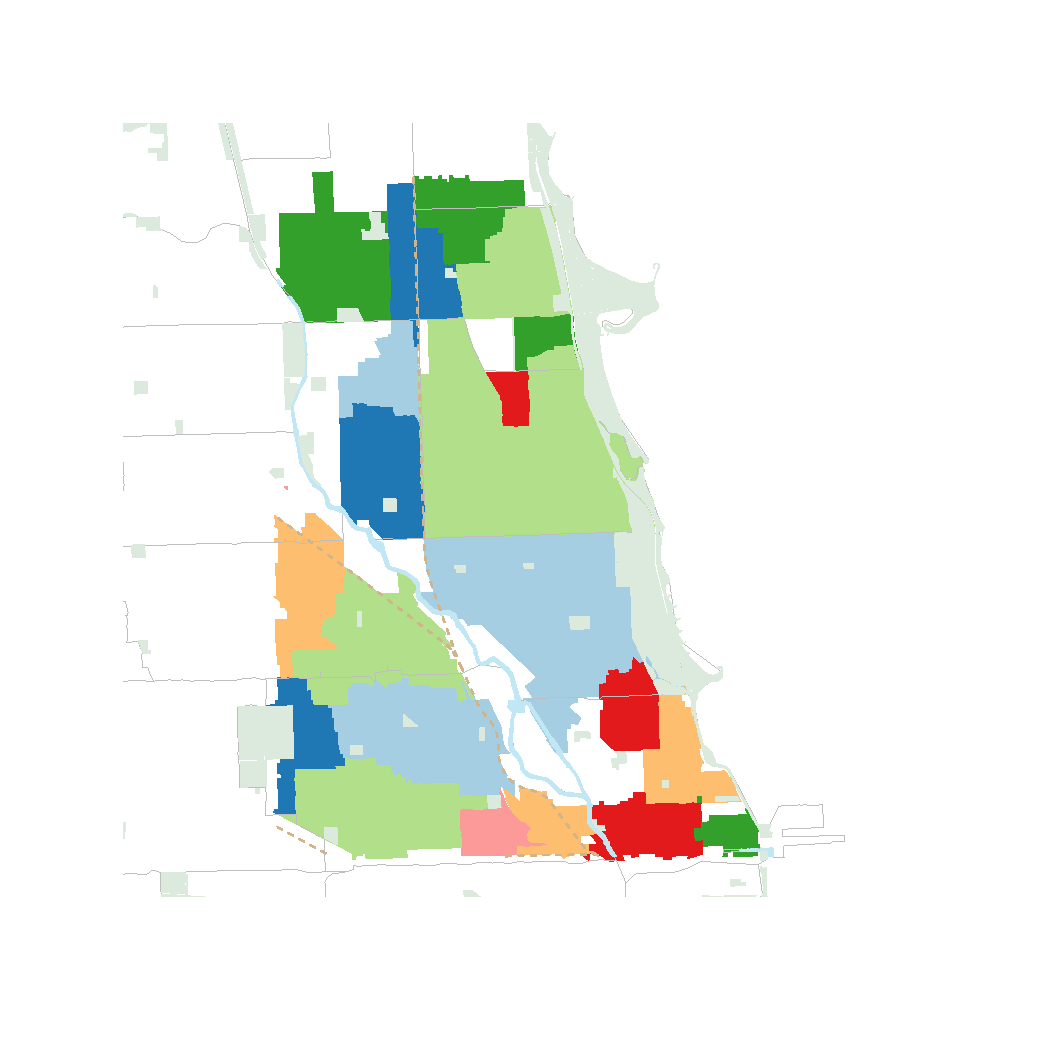
\includegraphics{./respect_grid.pdf}
\caption{Hand tuned smoothed neighborhoods}
\end{figure}

I would like to treat this measure as a kind of `averaged neighborhood
perception.' Of course, it's biased measure of that. There are
enormous selection effects, but perhaps more troublesome is that
listers are likely to choose neighborhood claims strategically in
order to make a listing maximally desirable. I have been looking for
scientific samples of neighborhood perception that I can compare
against so as to get a sense of magnitude of the biases.

However, I think it's possible that these data, with their biases
might be good enough, and we'll have ways of checking that. 

In addition to these data about neighborhood perception, we also have
block level census data as well as a trove of unaggregated data from
the City of Chicago on the built environment, crimes, 311 reports,
zoning, and the similar. We'd like to set them in relation to each
other.

\section*{Data Details}
The ultimate units of measurement are U.S. Census blocks the edges
between them. The U.S. Census blocks mainly correspond to city face
blocks. We use a rook adjacency to define the edges, i.e. all edges
are between blocks that share a common border of length greater than
0. In the training data, there are 5,857 blocks and
  13,887 edges.

For the inter-block similarities, we will use physical, demographic,
and administrative features.

\subsection*{Physical Barriers}
Highways, rail lines, rivers, and major streets can act as convenient
neighborhood boundaries. For each of these types of features, we code
an edge feature variable as 1 if the two adjacent blocks are separated
by the feature or code and 0 otherwise.

We also measure the difference in orientation between blocks. Blocks
are nearly all longer than they are wide, and we calculate the angle
of the longest side. For each edge, we calculate the difference
between the orientations of the blocks. We normalize the difference to
fall in $[0,1]$. 

\subsection*{School Boundaries}
If two adjacent blocks are in different elementary school attendance
boundary then we code an edge feature with 1, 0 otherwise. Similar for
high schools.

\subsection*{Demographic Features}

From the U.S. Census, we have block level information on race, age,
family structure, and housing ownership patterns. We can define
measures between blocks for these data. 

The measure we will use is the Jensen Shannon Divergence, which is a
symmetric measure of the similarity of distributions that ranges from
0 to 1. 

For race, the distribution is the number people coded by the Census as
``Hispanic or Latino'', ``Not Hispanic or Latino : White alone'',
``Not Hispanic or Latino : Black Alone'', and ``Not Hispanic or Latino
: Asian alone.'' 

For age, the distribution is the number of people
under 5, between 5 and 17, between 18 and 20, between 21 and 29,
between 30 and 64, and over 85. These age ranges were chosen to
capture life stages that tend to be spatially segregated: preschool,
school age, college age, young adult, middle age, retired. 

For family structure, the distribution is ``Husband-wife family'',
``Male householder, no wife present'', ``Female householder, no
husband present'', ``Householder, living alone'', and ``Householder,
not living alone''.

Many blocks have no one living in them or only a handful. In such
cases, it makes little sense to compare say racial composition. If
either adjacent blocks has fewer than 30 persons living in it, we do
not calculate the Jensen-Shannon divergences. There are
7,142 edges where we calculate these
demographic similarities.


\begin{kframe}


{\ttfamily\noindent\color{warningcolor}{\#\# Warning: argument is not numeric or logical: returning NA}}\end{kframe}% latex table generated in R 3.0.2 by xtable 1.7-1 package
% Wed Jan  8 11:09:45 2014
\begin{table}[ht]
\centering
\begin{tabular}{rrrrrrr}
  \hline
 & Mean & Min & 25th Quant. & Median & 75th Quant. & Max \\ 
  \hline
sufficient.population & 0.51 &  &  &  &  &  \\ 
  rail & 0.01 &  &  &  &  &  \\ 
  highway & 0.02 &  &  &  &  &  \\ 
  water & 0.01 &  &  &  &  &  \\ 
  zoning &  &  &  &  &  &  \\ 
  elementary.school & 0.09 &  &  &  &  &  \\ 
  high.school & 0.03 &  &  &  &  &  \\ 
  grid.street & 0.17 &  &  &  &  &  \\ 
  age.js & 0.05 & 0.00 & 0.02 & 0.04 & 0.06 & 0.69 \\ 
  race.js & 0.04 & 0.00 & 0.01 & 0.02 & 0.05 & 0.61 \\ 
  housing.js & 0.02 & 0.00 & 0.00 & 0.01 & 0.02 & 0.31 \\ 
  block.angle & 0.18 & 0.00 & 0.00 & 0.00 & 0.50 & 0.98 \\ 
  family.js & 0.06 & 0.00 & 0.02 & 0.04 & 0.07 & 0.60 \\ 
   \hline
\end{tabular}
\end{table}



\begin{figure}
\begin{knitrout}
\definecolor{shadecolor}{rgb}{0.969, 0.969, 0.969}\color{fgcolor}

{\centering \includegraphics[width=\maxwidth]{/home/fgregg/sweave-cache/figs/railImage} 

}



\end{knitrout}

\caption{Rail Lines}
\end{figure}

\begin{figure}
\begin{knitrout}
\definecolor{shadecolor}{rgb}{0.969, 0.969, 0.969}\color{fgcolor}

{\centering \includegraphics[width=\maxwidth]{/home/fgregg/sweave-cache/figs/highwayImage} 

}



\end{knitrout}

\caption{Highways}
\end{figure}

\begin{figure}
\begin{knitrout}
\definecolor{shadecolor}{rgb}{0.969, 0.969, 0.969}\color{fgcolor}

{\centering \includegraphics[width=\maxwidth]{/home/fgregg/sweave-cache/figs/gridImage} 

}



\end{knitrout}

\caption{Major Streets}
\end{figure}

\begin{figure}
\begin{knitrout}
\definecolor{shadecolor}{rgb}{0.969, 0.969, 0.969}\color{fgcolor}

{\centering \includegraphics[width=\maxwidth]{/home/fgregg/sweave-cache/figs/waterImage} 

}



\end{knitrout}

\caption{River}
\end{figure}

\begin{figure}
\begin{knitrout}
\definecolor{shadecolor}{rgb}{0.969, 0.969, 0.969}\color{fgcolor}

{\centering \includegraphics[width=\maxwidth]{/home/fgregg/sweave-cache/figs/elementaryImage} 

}



\end{knitrout}

\caption{Elementary School Attendance Boundaries}
\end{figure}

\begin{figure}
\begin{knitrout}
\definecolor{shadecolor}{rgb}{0.969, 0.969, 0.969}\color{fgcolor}

{\centering \includegraphics[width=\maxwidth]{/home/fgregg/sweave-cache/figs/highschoolImage} 

}



\end{knitrout}

\caption{High School Attendance Boundaries}
\end{figure}

\begin{figure}
\begin{knitrout}
\definecolor{shadecolor}{rgb}{0.969, 0.969, 0.969}\color{fgcolor}

{\centering \includegraphics[width=\maxwidth]{/home/fgregg/sweave-cache/figs/zoningImage} 

}



\end{knitrout}

\caption{Zoning Differences}
\end{figure}

\begin{figure}
\begin{knitrout}
\definecolor{shadecolor}{rgb}{0.969, 0.969, 0.969}\color{fgcolor}

{\centering \includegraphics[width=\maxwidth]{/home/fgregg/sweave-cache/figs/sufficientImage} 

}



\end{knitrout}

\caption{Sufficient Population}
\end{figure}


\begin{figure}
\begin{knitrout}
\definecolor{shadecolor}{rgb}{0.969, 0.969, 0.969}\color{fgcolor}

{\centering \includegraphics[width=\maxwidth]{/home/fgregg/sweave-cache/figs/blockAngleImage} 

}



\end{knitrout}

\caption{Difference in Block Orientation}
\end{figure}

\begin{figure}
\begin{knitrout}
\definecolor{shadecolor}{rgb}{0.969, 0.969, 0.969}\color{fgcolor}

{\centering \includegraphics[width=\maxwidth]{/home/fgregg/sweave-cache/figs/_raceImage} 

}



\end{knitrout}

\caption{Difference in Distribution of Race and Ethnicity}
\end{figure}


\begin{figure}
\begin{knitrout}
\definecolor{shadecolor}{rgb}{0.969, 0.969, 0.969}\color{fgcolor}

{\centering \includegraphics[width=\maxwidth]{/home/fgregg/sweave-cache/figs/_ageImage} 

}



\end{knitrout}

\caption{Difference in Distribution of Age}
\end{figure}


\begin{figure}
\begin{knitrout}
\definecolor{shadecolor}{rgb}{0.969, 0.969, 0.969}\color{fgcolor}

{\centering \includegraphics[width=\maxwidth]{/home/fgregg/sweave-cache/figs/_familyImage} 

}



\end{knitrout}

\caption{Difference in Distribution of Family Type}
\end{figure}


\begin{figure}
\begin{knitrout}
\definecolor{shadecolor}{rgb}{0.969, 0.969, 0.969}\color{fgcolor}

{\centering \includegraphics[width=\maxwidth]{/home/fgregg/sweave-cache/figs/_housingImage} 

}



\end{knitrout}

\caption{Difference in Distribution of Housing Type}
\end{figure}

\section*{Results}

% latex table generated in R 3.0.2 by xtable 1.7-1 package
% Wed Jan  8 13:06:03 2014
\begin{table}[ht]
\centering
\begin{tabular}{rrr}
  \hline
 & no\_pop & pop \\ 
  \hline
(Intercept) & 0.0019 & 0.0006 \\ 
  Railroad & 0.0253 & 0.0255 \\ 
  Water & 0.0130 & 0.0166 \\ 
  Highway & 0.0057 &  \\ 
  Major Street & 0.0065 & -0.0206 \\ 
  Elementary School & 0.0103 & 0.0110 \\ 
  High School & 0.0084 & 0.0104 \\ 
  Block Angle & -0.0144 & -0.0263 \\ 
  Family Structure &  & -0.0017 \\ 
  Race and Ethnicity &  & 0.0022 \\ 
  Age Structure &  & -0.0032 \\ 
  Housing Structure &  & -0.0012 \\ 
   \hline
\end{tabular}
\end{table}




\begin{figure}
\begin{knitrout}
\definecolor{shadecolor}{rgb}{0.969, 0.969, 0.969}\color{fgcolor}

{\centering \includegraphics[width=\maxwidth]{/home/fgregg/sweave-cache/figs/plotPredictions} 

}



\end{knitrout}

\caption{Predicted Neighborhoods}
\end{figure}


\begin{figure}
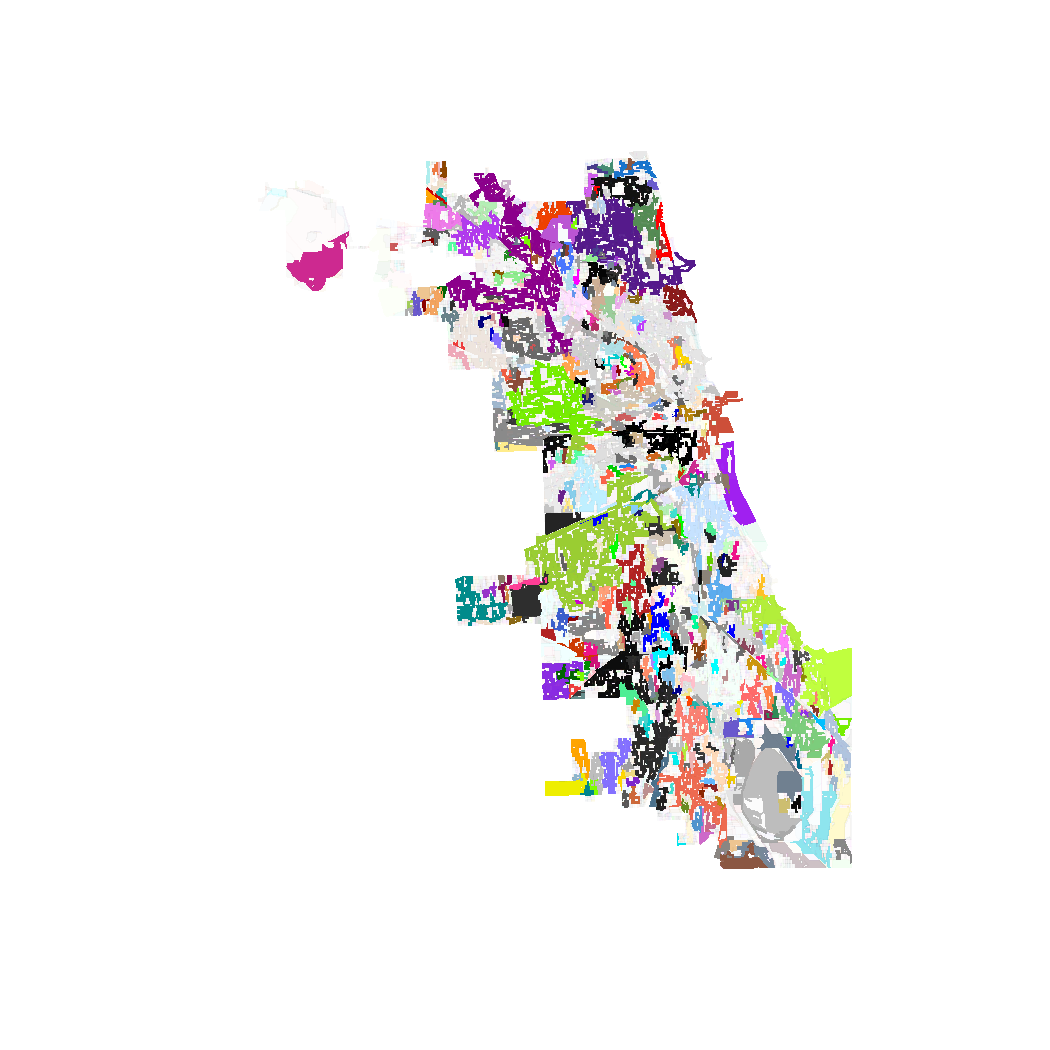
\includegraphics{../code/training/predicted_chicago_neighborhoods.pdf}
\end{figure}


TODO rand index on community measures

\end{document}
